\chapter{Introduction}
\label{c:introduction}

The Indian Summer Monsoon (hereafter also referred to as ISM\footnote{An overview over all abbreviations used in this work can be found in \cref{apx:abbreviations}.}) is one of the most significant meteorological events on our planet. Each year during the time-frame from June to September, it shapes the lives of the more than one billion people living on the Indian subcontinent. Stretching from the Tibetan Plateau and the Himalayas up north down to the coasts of the Indian Ocean, the Indian subcontinent is an enormous geographical area that encompasses countries like India, Pakistan and Bangladesh, amongst others. The terms ``Indian subcontinent'' and ``South Asia'' are often used interchangeably, even though they are both only loosely defined.

\begin{figure}[h]
  \centering
  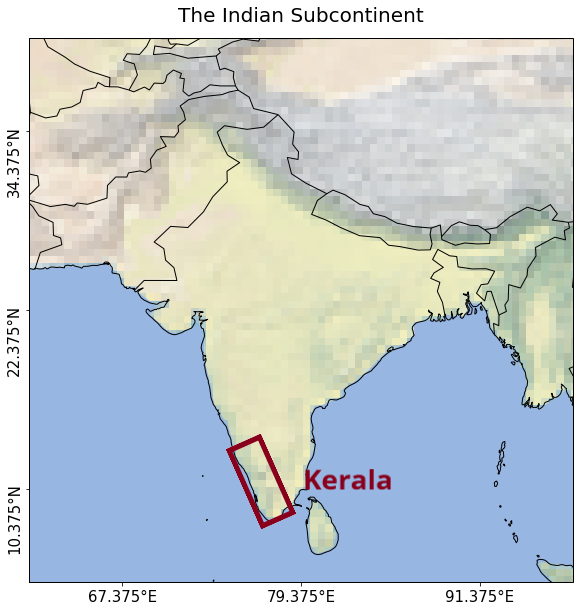
\includegraphics[width=0.3\linewidth]{./99_appendix/img/area_overview_kerala}
  \caption{Geographical area of the Indian subcontinent as used in our work. Kerala, a region especially important for the prediction of ISM onset, is emphasized in red.}
  \label{fig:the_indian_subcontinent}
\end{figure}

As illustrated in \Cref{fig:the_indian_subcontinent}, India makes up for a major portion of the Indian subcontinent (hence the matching naming). Due to it being one of the most highly populated countries on earth, as well as one of the first to be impacted by the yearly occurrence of the ISM, we focus our work mainly on the ramifications of the ISM on India and its general population.

The ISM is of great importance to the Indian population: many parts of India receive up to 80\% of rainfall during the monsoon season, and significant parts of the population obtain their drinking water from monsoon rainfalls \citep{Stolbova.2015}. Farmers further depend on the arrival of these rainfalls to be able to water their crops and feed their livestock. The monsoon is of similarly high impact for the Indian economy at large, as the agricultural sector makes up almost one-fifth of India's gross-domestic product (GDP) \citep{CentralIntelligenceAgency.05.01.2018}.

In itself, the ISM is a highly complex climatological phenomenon. It displays considerable variability in both timing and strength and is influenced by many factors on regional and global scales. Due to its evident importance, the behavior of the ISM has been a focus of climate researchers for many decades, bringing to light many theories and hypotheses. Numerous approaches for the prediction of monsoon onset and withdrawal, the times at which monsoon weather conditions reach and leave a particular location, have been proposed over the years. Other research seeks to analyze and predict the amount of rainfall that locations in India get during the monsoon season, which could allow the population to better prepare for the potential dangers of extreme rainfall.

Many factors that drive the ISM are still unknown or unexplained, even after many years of research. Prediction tasks tend to be hard to accomplish and rely on sophisticated climatological models, while their accuracy is often subpar when compared with weather prediction in ``more predictable'' countries in Europe or North America. The India Meteorological Department (IMD), the agency that is officially tasked with the analysis and prediction of ISM behavior, predicts the monsoon from up to a one month lead and manages to do so with a root mean-squared error (RMSE) of about four days \citep{Pradhan.2017}. However, it has regularly failed to predict even drought-like conditions \citep{Paliwal.24.09.2017}.

A problem in prediction tasks is often the computing power that is needed to drive accurate models for complex phenomena. More data than ever before is being collected by satellites and sensors every day, resulting in high computational requirements. Additionally, climatological phenomena are ever-changing and are subject to large-scale trends like climate change, making successful predictions even harder to accomplish. Recent climatic trends tend to further increase the variability of natural phenomena like rainfall, resulting in increased numbers of droughts as well as extreme rainfall events in India. The tremendous impact of the climate on the welfare of society and the economy at large makes having the capability to predict weather events accurately, be it rainfall, drought or the monsoon onset, more crucial than ever.

The availability and affordability of computing resources have been increasing at a very fast pace during the last decade, leading to the emergence of many sophisticated methods for data analysis and prediction. Neural networks, a category of machine learning models that has its origins in the early 20th century, have only become practical during recent years, as the amount of data and computational power required to train them adequately had never been available before. Since the reemergence of neural networks, they have become a key component in complicated machine learning tasks like image recognition and natural language processing. As they even seem to be able to learn patterns in data that humans do not know of yet, they could be a good contender for tasks like the prediction of ISM behavior. However, the application of neural networks and deep learning in this climatological domain is not yet as prevalent as it is in classical computer science domains.

In this work, we seek to evaluate the applicability of the aforementioned neural networks to the domain of ISM onset prediction. In addition, we analyze the spatial and temporal distribution of extreme rainfall during the different seasons of monsoon. Because of the complex behavior of the ISM, we dedicate \cref{c:ism_overview} of this work to a short summarization of research about the inner workings of the ISM. We explain the major factors that are known to influence monsoon and try to further motivate the significance and social impact of the monsoon for the people in India and its surrounding countries.

The remainder of this work is structured into two major parts: the first part (\cref{c:event_sync}) is dedicated to the analysis of extreme rainfall events before, during and after the monsoon season. Such events are regularly seen all over India and represent one of the most significant challenges the local population faces from the ISM. Extreme rainfall can cause enormous damage by flooding cities or destruction of essential infrastructure. As such, there is a clear need to analyze and predict the spatial and temporal distribution of these extreme rainfall events.

Basing our first part on the work of \citet{Stolbova.2015}, we closely follow her methodology and choice of dataset: all work in \cref{c:event_sync} is based on the Tropical Rainfall Measurement Mission (TRMM) dataset, a precipitation dataset compiled by the National Aeronautics and Space Agency (NASA) and the Japanese Aerospace Exploration Agency (JAXA). The TRMM product we use in this work contains data for the years 1998-2016 at a {0.25\degree} resolution. Because of its high resolution, the TRMM dataset is a popular choice for climate research whenever a high level of detail is needed.

As a first step in the analysis of the aforementioned TRMM dataset, we extract extreme rainfall events and build event series for different locations in India. We then calculate the synchronicity of different pairs of locations\footnote{Simplified example: two locations are synchronous if an extreme event in one location tends to be followed by an extreme event in the other location.} and build a ``climate network'' connecting only the most significantly synchronous locations.

Analysis of the resulting network using network centrality measures finally gives us an intuition about the importance of a location the network. In this work, we use several different measures: firstly, we calculate the degree of locations, giving us the number of locations to which a location is synchronous. Secondly, the betweenness of a location gives us the number of shortest paths between locations that this location lies on. And finally, the PageRank algorithm, which has been created by Larry Page and Sergey Brin to calculate the importance of web pages in their search engine Google. Knowledge about these measures could potentially help in the analysis or even prediction of monsoon behavior. For example, extreme rainfall in a location that is very central might be a reason to implement safety measures in connected locations.

The second part of this work (\cref{c:part2}) deals with the critical issue of monsoon onset prediction. The onset date for a location in India depicts the point at which the monsoon reaches said location with strength and durability above a predefined threshold. We try to predict such an onset date for the Kerala region on the southern tip of the Indian subcontinent (as shown in \cref{fig:the_indian_subcontinent}), which is one of the first locations reached by the ISM and as such marks the beginning of monsoon for the whole Indian subcontinent.

We base our onset prediction task on two climate datasets: in addition to the TRMM dataset we have already introduced, we use the ERA-Interim dataset as produced by the European Centre for Medium-Range Weather Forecasts (ECMWF). Starting in 1979, ERA-Interim is available for a longer period than TRMM but at a much less detailed {0.75\degree} resolution. In contrast to the TRMM dataset, which is purely focused on the amount of precipitation, ERA-Interim contains many different features (e.g., temperature) at various vertical levels (measured according to their pressure).

Based on the datasets as mentioned earlier, we build neural network architectures using the Python Keras 2.0 and Tensorflow 1.4 libraries, describing the intuition of each. Experiments with each model allow us to evaluate and shortly summarize our most important findings. We iteratively improve upon the findings of each model, building models with vastly different architectures as well as for a number features and combinations thereof (TRMM, ERA-Interim, different sets of onset dates). An overview and comparison of the learning capabilities of all models serve as a conclusion to the second part.

Finally concluding our work in \cref{c:conclusion}, we summarize our overall findings and reflect on the results of \cref{c:event_sync} and \cref{c:part2}. We additionally provide ideas for the improvement of our work and possible future research based on the topics of extreme event synchronization and monsoon onset prediction using deep learning methods.
